\documentclass{beamer}

% You can uncomment the themes below if you would like to use a different
% one:
%\usetheme{AnnArbor}
%\usetheme{Antibes}
%\usetheme{Bergen}
% \usetheme{Berkeley}
%\usetheme{Berlin}
%\usetheme{Boadilla}
%\usetheme{boxes}
%\usetheme{CambridgeUS}
%\usetheme{Copenhagen}
%\usetheme{Darmstadt}
%\usetheme{default}
%\usetheme{Frankfurt}
%\usetheme{Goettingen}
%\usetheme{Hannover}
%\usetheme{Ilmenau}
%\usetheme{JuanLesPins}
%\usetheme{Luebeck}
\usetheme{Madrid}
%\usetheme{Malmoe}
%\usetheme{Marburg}
%\usetheme{Montpellier}
%\usetheme{PaloAlto}
%\usetheme{Pittsburgh}
%\usetheme{Rochester}
%\usetheme{Singapore}
%\usetheme{Szeged}
% \usetheme{Warsaw}

\usepackage{kotex} % For using korean. Do not modify this line.
\usepackage{listings} % For embedding codes. Do not modifiy this line. 

\usepackage{datetime} % For using date at compile time. 

\logo{{
\includegraphics[height=0.7cm]{../../References/Template Images/fastcampus-logo-positive.png}}}

% slide environment 
\newenvironment{slide}[1][]
{%
  \begin{frame}[allowframebreaks,#1]%
  }{%
  \end{frame}%
}
% \newcounter{totalcontinuationcount}
% \makeatletter
% \setbeamertemplate{frametitle continuation}{%
    % \setcounter{totalcontinuationcount}{\beamer@endpageofframe}%
    % \addtocounter{totalcontinuationcount}{1}%
    % \addtocounter{totalcontinuationcount}{-\beamer@startpageofframe}%
    % \ifnum \value{totalcontinuationcount} > 1
        % \textmd{(\insertcontinuationcount/\arabic{totalcontinuationcount})}%
    % \fi
% }
% \makeatother
\setbeamertemplate{frametitle continuation}[from second][\insertcontinuationcountroman]

% Code embeddings 

\renewcommand{\lstlistingname}{Code}
\renewcommand{\lstlistlistingname}{List of \lstlistingname s}

\newcommand{\includecode}[3]{\lstinputlisting[caption=#3, style=#1]{#2}} % For code inclusion. 

\newcommand{\python}[2]{\lstinputlisting[caption=#2, style=python]{#1}} % For code inclusion. 

\newcommand{\cpp}[2]{\lstinputlisting[caption=#2, style=cpp]{#1}} % For code inclusion. 


\usepackage{color}
\definecolor{dkgreen}{rgb}{0,0.6,0}
\definecolor{gray}{rgb}{0.5,0.5,0.5}
\definecolor{mauve}{rgb}{0.58,0,0.82}

\lstdefinestyle{python}{frame=tb,
  language=Python,
  aboveskip=3mm,
  belowskip=3mm,
  showstringspaces=false,
  columns=flexible,
  basicstyle={\small\ttfamily},
  numbers=left,
  numberstyle=\tiny\color{gray},
  keywordstyle=\color{blue},
  commentstyle=\color{dkgreen},
  stringstyle=\color{mauve},
  breaklines=true,
  breakatwhitespace=true,
  tabsize=4
}

\lstdefinestyle{cpp}{frame=tb,
  language=C++,
  aboveskip=3mm,
  belowskip=3mm,
  showstringspaces=false,
  columns=flexible,
  basicstyle={\small\ttfamily},
  numbers=left,
  numberstyle=\tiny\color{gray},
  keywordstyle=\color{blue},
  commentstyle=\color{dkgreen},
  stringstyle=\color{mauve},
  breaklines=true,
  breakatwhitespace=true,
  tabsize=4
}


\title{Beamer Template for the Lecture Slides}

% A subtitle is optional and this may be deleted
\subtitle{Fastcampus Online Lecture}

\author{신승우}


% Let's get started
\begin{document}

\begin{slide}
  \titlepage
\end{slide}

\begin{slide}{Outline}
  \tableofcontents %[hideallsubsections]
  % You might wish to add the option [pausesections]
\end{slide}

% Section and subsections will appear in the presentation overview
% and table of contents.

\section{Basics} 

% \begin{slide}[fragile, environment=slide]{} 
% \end{slide}

\begin{slide}[fragile, environment=slide]{항목 나열} 

원하는 텍스트를 쓰면 됩니다. 일반적인 \LaTeX 문법에 대해서는 lecture notes의 template을 참조하세요.

\end{slide}

\begin{slide}[fragile, environment=slide]{항목 나열} 

\begin{itemize} 
\item itemize 환경과 item을 이용하여 항목을 나열할 수 있습니다. 
\begin{itemize} 
\item 이렇게 subitem도 만들 수 있습니다. 
\end{itemize}
\item Empty Text 
\end{itemize}
\end{slide}


\section{Useful Environments}

\begin{slide}[fragile, environment=slide]{Definitions} 
정의는 다음과 같이 작성합니다. 

\begin{definition}{Definition} 
정의 환경은 \textbf{definition}이며, textbf를 이용하여 정의 내에서 특정 단어를 강조할 수 있습니다. 
\end{definition}

\end{slide}

\begin{slide}[fragile, environment=slide]{Equation} 

\begin{itemize}
\item Inline equation은 $1+1$과 같이, 달러 표시를 이용합니다. 
\item 따로 항목을 가지는 equation은 다음과 같이 사용합니다. 
\end{itemize} 

\begin{equation} 
a = b+c
\end{equation}

\end{slide}

\begin{slide}[fragile, environment=slide]{행렬}
행렬은 다음과 같이 작성합니다. 

$ \left[ \begin{matrix}
0 & 1  \\
1 & 0 
\end{matrix} \right]$  
\end{slide}


\section{Figures and Tables} 

\begin{slide}[fragile, environment=slide]{Include Figures : Using Tikz} 

\LaTeX은 그림을 그리는 자체 라이브러리 tikz를 제공합니다. 이 라이브러리를 이용하여 그림을 그리는 것에 대해서는 다른 매뉴얼을 참고하시길 바랍니다. 

\end{slide}

\begin{slide}[fragile, environment=slide]{Include Figures : Using File} 
그림은 includegraphics 명령어를 이용하여 삽입할 수 있습니다. 
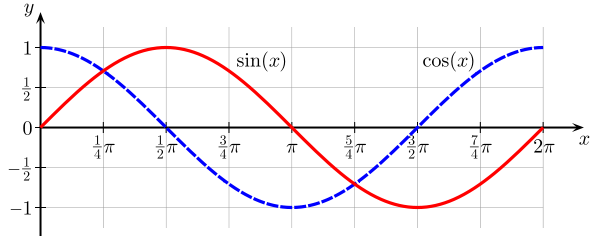
\includegraphics[width=\textwidth]{cos}
\end{slide}

\begin{slide}[fragile, environment=slide]{표 만들기}
표는 가능하면 손으로 만들지 말고, \href{https://www.tablesgenerator.com/}{table generator} 사이트를 이용하여 만들기 바랍니다. 

\begin{table}[]
\centering
\caption{$x*(y+z)$ 체크}
\label{my-label}
\begin{tabular}{|l|l|l|}
\hline
current string & rule & result \\ \hline
x*(y+z)&1    & is x part?, is * binary?, is (y+z) part?      \\ \hline
x &  2, 3 & x is num! / num is part!      \\ \hline
*& 3    & * is binary!      \\ \hline
(y+z)& 3    &  is y+z expr?      \\ \hline
y, z& same to x    &   y,z is num! / num is part!   \\ \hline
+ & 3    &  + is binary!     \\ \hline
\end{tabular}
\end{table}

\end{slide} 

\section{Code Embeddings}

\begin{slide}[fragile, environment=slide]{Code Embedding : Python} 

코드는 다음과 같이 언어를 특정하여 넣을 수 있습니다. 

\begin{lstlisting} [style=Python]
print("hello world!")
\end{lstlisting}

\begin{lstlisting} [style=cpp]
cout << "hello world!"
\end{lstlisting}
\end{slide}


\begin{slide}[fragile, environment=slide]{Code Embedding from File : Python} 
원하는 외부 파일을 참조하고 싶은 경우, 아래와 같이 합니다. 
\python{hello.py}{hello world!}
\framebreak
\includecode{python}{hello.py}{hello world!}
\end{slide}

\begin{slide}[fragile, environment=slide]{Code Embedding from File : C++} 
\cpp{hello.cpp}{hello world!}
\framebreak
\includecode{cpp}{hello.cpp}{hello world!}
\end{slide}

\end{document}


